\chapter{Onion Routing}
\label{chap:Capitolo1}

\begin{figure}
    \centering
    \def\svgwidth{\columnwidth}{SpiegazioneOnion}
    % 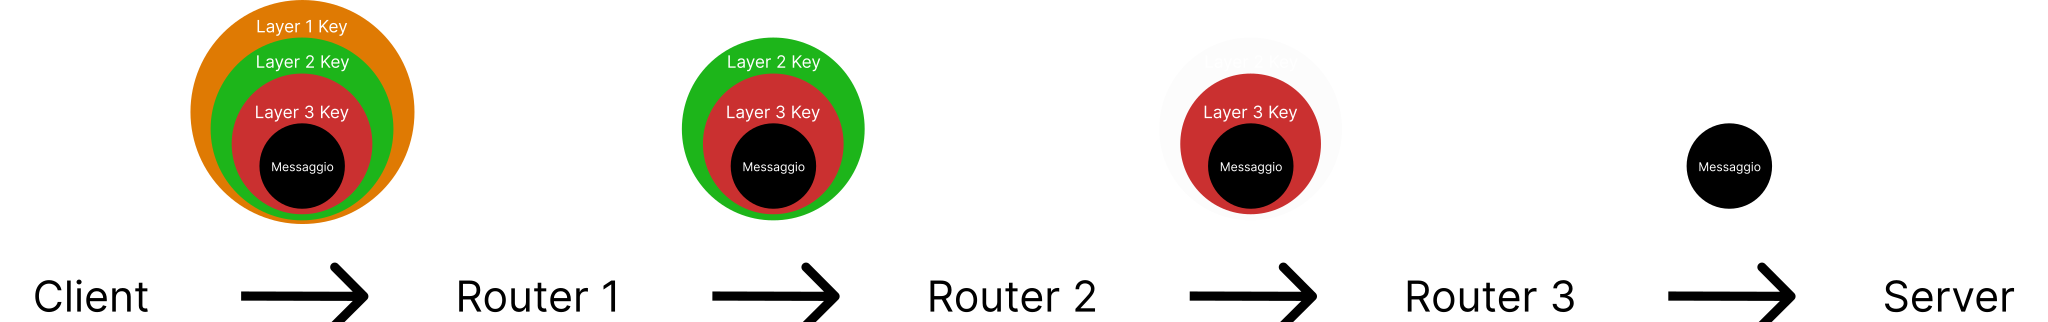
\includegraphics[width=0.5\textwidth]{SpiegazioneOnion}
    \caption{Vita di un messaggio onion}
    \label{fig:routing}
\end{figure}
La rete onion è una rete distribuita composta dall'insieme di router onion che agiscono come nodi di rete e collaborano per portare un pacchetto dalla sorgente alla destinazione. Il tutto avviene senza che nessun nodo possa conoscere contemporaneamente l'host sorgente e l'host di destinazione, grazie alla criptografia a strati del pacchetto, per cui ogni strato viene criptato con una chiave differente e può essere decriptato solo dal nodo con la stessa chiave simmetrica, scoprendo cosi le informazioni sul prossimo nodo. Il nodo finale (exit node) può infine decriptare l'intero messaggio e scoprirne il corpo. Questo meccanismo è derivato dallo studio di David Chaum riguardo alle mix networks. La risposta del pacchetto segue lo stesso criterio sfruttando nodi, algoritmi e chiavi differenti. Questo concede all'utilizzatore di rimanere completamente anonimo, cosa che non può essere avvenire con la semplice criptografia SSL che agisce esclusivamente sul corpo del messaggio
Come prima operazione per utilizzare la rete onion il client deve generare un nuovo circuito definendo il percorso di nodi che ogni pacchetto dovrà seguire, iniziando dal primo nodo vengono scambiate informazioni crittografiche come l'algoritmo e le chiavi da usare, poi si usano le informazioni finora ottenute per ottenere quelle del prossimo nodo e cosi via fino a che non si è generato tutto il circuito, grazie a questo meccanismo neanche durante la generazione del circuito è possibile risalire al client. Viene usata la crittografia asimmetrica per scambiare le chiavi simmetriche tra il client e ogni router, questo viene fatto in quanto la crittografia asimmetrica è molto costosa e viene quindi usata solo alla generazione del circuito, successivamente gli strati vengono criptati e decriptati con la stessa chiave simmetrica. Questo consente alla rete onion ad avere una bassa latenza che è incrementata solo dal numero di onion router nel percorso e non dalla tecnologia che non è distante da quella usata in HTTPS



\section{Applicazioni di utilizzo}
L’onion routing può essere usato con una moltitudine di protocolli e applicazioni, tra i più comuni troviamo HTTP(S), FTP, SSH, SMTP, DNS e VPNs. L’utilizzo di molti dei protocolli più comuni avviene tramite gli onion proxies, i quali sono suddivisi in tre proxy layer logici
- Un proxy che genera e gestisce le connessioni, per operare ha necessità di conoscere la topologia e i percorsi verso altri nodi, tutte le informazioni vengono distribuite in modo sicuro all’interno della rete a ogni nuovo nodo che si connette 
- Un proxy chiamato “Application Specific Proxy”, a una connessione la relativa applicazione invia al proxy il pacchetto che normalmente invierebbe al server di destinazione, il proxy si occupa di convertire lo stream di dati in un formato accettato dalla rete onion
- Un proxy opzionale chiamato “Application Specific Privacy Filter” che sanifica lo stream di dati rimuovendo informazioni che potrebbero identificare la sorgente[1]
I proxy possono essere configurati in molteplici modi, tra i quali vi è la possibilità di eseguire il software proxy in un server remoto e sfruttare la rete tor da ogni dispositivo senza dover installare il software in ogni dispositivo, che quindi non ne deve gestire la computazione

 
\section{Tor ~ Onion v2}
Nel 2002 viene presentata la rete Tor, diventata open source 2 anni dopo è l’implementazione più famosa di onion routing che porta alcuni miglioramenti sostanziali
Migliore segretezza del canale, nella versione originale un nodo poteva forzare altri onion router nel circuito a decriptare il traffico precedentemente registrato. La rete tor sfrutta una tecnica di circuiti telescopici in cui il client che genera il circuito crea chiavi di sessione di breve durata che quindi non potranno essere usate dai malintenzionati per decriptare il vecchio traffico
L’implementazione del proxy di applicazione attraverso lo standard SOCKS, consente alla maggior parte del traffico TCP di funzionare senza modifiche. Precedentemente era necessario implementare un proxy per ogni applicazione, era quindi necessario generare un circuito per ogni applicazione, con conseguente duplicazione di chiavi, in Tor invece il circuito viene generato a livello di TCP e più applicazioni possono sfruttarlo. Per garantire la non tracciabilità di un utente nello stesso stream dati usato da più applicazioni è stato implementato il meccanismo dei rotating circuits che genera ogni minuto un nuovo circuito se quello precedente non viene usato
Controllo di congestione, un sistema decentralizzato che sfrutta ack end-to-end per garantire l’anonimato
Directory Server, nodi più fidati di altri che descrivono le informazioni di rete in maniera sicura e affidabile
Politiche di uscita variabili, ogni nodo possiede delle politiche che specificano le connessioni consentite e rifiutate, fondamentale in una rete distribuita fatta da volontari
Controllo di integrità end-to-end, viene eseguito un controllo di integrità nel momento in cui il pacchetto esce dalla rete per garantire che i contenuti non sono stati alterati
Tor, a differenza degli altri sistemi che implementano le Mix-Network di Chaum predilige la bassa latenza, il che rende la rete adatta all’utilizzo tramite un web browser, questo inoltre migliora l’usabilità di tor il che è un aspetto fondamentale dato che maggiori sono i nodi e più semplice garantire l’anonimato.
Tor non è completamente sicuro, infatti non filtra informazioni di privacy nel corpo del messaggio come invece avviene in altri sistemi come Privoxy o Anonymizer e non offre garanzie in caso di attacco end-to-end che concerne sia sorgente che destinazione 